\documentclass[12pt,a4paper]{article}

% ─── Packages ────────────────────────────────────────────────────────────────
\usepackage[margin=2.5cm, headheight=15pt]{geometry}
\usepackage{fontenc}
\usepackage{inputenc}
\usepackage{lmodern}
\usepackage{microtype}
\usepackage{graphicx}
\usepackage{xcolor}
\usepackage{booktabs}
\usepackage{longtable}
\usepackage{array}
\usepackage{tabularx}
\usepackage{multirow}
\usepackage{hhline}
\usepackage{listings}
\usepackage{fancyhdr}
\usepackage{titlesec}
\usepackage{tocloft}
\usepackage{hyperref}
\usepackage{amsmath}
\usepackage{amssymb}
\usepackage{enumitem}
\usepackage{mdframed}
\usepackage{tikz}
\usetikzlibrary{shapes.geometric, arrows.meta, positioning, calc, fit, backgrounds}
\usepackage{colortbl}
\usepackage{float}
\usepackage{caption}
\usepackage{subcaption}

% ─── Colours ─────────────────────────────────────────────────────────────────
\definecolor{zaraigreen}{RGB}{34,139,34}
\definecolor{zaraigold}{RGB}{184,134,11}
\definecolor{codebg}{RGB}{245,247,250}
\definecolor{codeborder}{RGB}{180,190,200}
\definecolor{sectioncolor}{RGB}{24,90,40}
\definecolor{tableheader}{RGB}{34,139,34}
\definecolor{linkcolor}{RGB}{0,80,160}
\definecolor{noteblue}{RGB}{230,240,255}
\definecolor{noteblueborder}{RGB}{100,150,220}

% ─── Hyperref ────────────────────────────────────────────────────────────────
\hypersetup{
  colorlinks=true,
  linkcolor=linkcolor,
  urlcolor=linkcolor,
  citecolor=linkcolor,
  pdftitle={ZaraiLink Search Engine Infrastructure},
  pdfauthor={ZaraiLink Engineering Team},
  pdfsubject={Technical Architecture Report}
}

% ─── Section formatting ───────────────────────────────────────────────────────
\titleformat{\section}
  {\Large\bfseries\color{sectioncolor}}
  {\thesection}{1em}{}[\vspace{-4pt}\textcolor{zaraigreen}{\rule{\linewidth}{1.5pt}}]

\titleformat{\subsection}
  {\large\bfseries\color{sectioncolor}}
  {\thesubsection}{1em}{}

\titleformat{\subsubsection}
  {\normalsize\bfseries\color{sectioncolor}}
  {\thesubsubsection}{1em}{}

% ─── Header / Footer ─────────────────────────────────────────────────────────
\pagestyle{fancy}
\fancyhf{}
\fancyhead[L]{\small\textcolor{zaraigreen}{\textbf{ZaraiLink}} --- Search Engine Infrastructure}
\fancyhead[R]{\small Technical Report}
\fancyfoot[C]{\small\thepage}
\renewcommand{\headrulewidth}{0.4pt}
\renewcommand{\footrulewidth}{0.4pt}

% ─── Code listing style ───────────────────────────────────────────────────────
\lstset{
  backgroundcolor=\color{codebg},
  basicstyle=\ttfamily\small,
  breakatwhitespace=false,
  breaklines=true,
  captionpos=b,
  commentstyle=\color{gray}\itshape,
  frame=single,
  framesep=4pt,
  rulecolor=\color{codeborder},
  keywordstyle=\color{blue}\bfseries,
  stringstyle=\color{teal},
  numberstyle=\tiny\color{gray},
  numbers=left,
  stepnumber=1,
  tabsize=2,
  language=Python,
  showstringspaces=false,
  xleftmargin=1em,
  xrightmargin=0.5em
}

% ─── Custom environments ──────────────────────────────────────────────────────
\newmdenv[
  backgroundcolor=noteblue,
  linecolor=noteblueborder,
  linewidth=1.5pt,
  roundcorner=4pt,
  skipabove=8pt,
  skipbelow=8pt,
  innerleftmargin=10pt,
  innerrightmargin=10pt
]{infobox}

% ─── Misc ─────────────────────────────────────────────────────────────────────
\setlength{\parskip}{6pt}
\setlength{\parindent}{0pt}

% ─────────────────────────────────────────────────────────────────────────────
\begin{document}
% ─── Title Page ───────────────────────────────────────────────────────────────
\begin{titlepage}
  \centering
  \vspace*{2cm}

  {\color{zaraigreen}\rule{\linewidth}{3pt}}
  \vspace{0.5cm}

  {\fontsize{28}{34}\selectfont\bfseries\color{sectioncolor}
    ZaraiLink Search Engine\\[6pt]Infrastructure
  }

  \vspace{0.3cm}
  {\large\color{gray} Technical Architecture \& Design Report}

  \vspace{0.3cm}
  {\color{zaraigreen}\rule{\linewidth}{1.5pt}}

  \vspace{2cm}

  % Pipeline diagram (TikZ) — 4 boxes, scaled to fit page width
  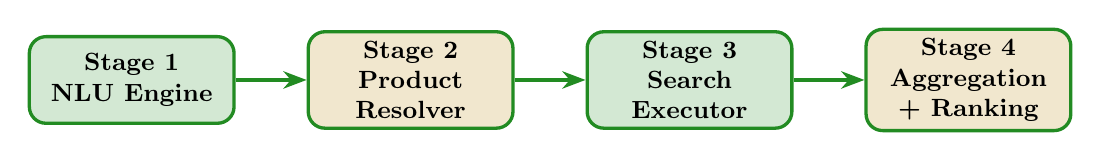
\begin{tikzpicture}[
    node distance=0.9cm,
    box/.style={rectangle, rounded corners=6pt, draw=zaraigreen,
                line width=1.2pt, minimum width=2.6cm, minimum height=1.1cm,
                align=center, font=\bfseries\small},
    arrow/.style={-Stealth, line width=1.2pt, color=zaraigreen}
  ]
    \node[box, fill=zaraigreen!20] (nlu)  {Stage 1\\NLU Engine};
    \node[box, fill=zaraigold!20,  right=of nlu]  (res)  {Stage 2\\Product\\Resolver};
    \node[box, fill=zaraigreen!20, right=of res]  (exec) {Stage 3\\Search\\Executor};
    \node[box, fill=zaraigold!20,  right=of exec] (rank) {Stage 4\\Aggregation\\+ Ranking};
    \draw[arrow] (nlu)  -- (res);
    \draw[arrow] (res)  -- (exec);
    \draw[arrow] (exec) -- (rank);
  \end{tikzpicture}

  \vspace{2.5cm}

  \begin{tabular}{ll}
    \textbf{Project:}   & ZaraiLink --- Agricultural Trade Intelligence Platform\\[4pt]
    \textbf{Component:} & Search \& Discovery Engine\\[4pt]
    \textbf{Stack:}     & Django 4.2, PostgreSQL, Redis, LightGBM, SentenceTransformers\\[4pt]
    \textbf{Version:}   & FYP Final Report\\[4pt]
    \textbf{Date:}      & April 27, 2026\\
  \end{tabular}

  \vfill

  {\color{zaraigreen}\rule{\linewidth}{3pt}}
  \vspace{0.3cm}
  {\small\color{gray}
    ZaraiLink Engineering Team $\cdot$ Habib University $\cdot$ FYP 2025--2026
  }
\end{titlepage}

% ─── Table of Contents ────────────────────────────────────────────────────────
\tableofcontents
\newpage

% ─────────────────────────────────────────────────────────────────────────────
\section{Executive Summary}

ZaraiLink is a Pakistani agricultural trade intelligence SaaS platform that aggregates
real government import/export transaction records and exposes them through a specialised
natural-language search interface.  The search engine is the platform's core value
proposition: it lets traders express intent in plain Urdu-inflected English (\emph{``cheapest
sugar from Brazil''}, \emph{``buyers for rice bulk 1000 mt''}) and receive a ranked list of
verified trading partners drawn directly from customs data.

The engine is designed around four sequential stages:

\begin{enumerate}[leftmargin=2cm]
  \item \textbf{NLU Engine} --- Extracts structured intent, products, country, price and
        quantity signals from a raw free-text query using a hybrid of regex rules, fine-tuned
        ML classifiers and a large-language-model (LLM) fast-path.
  \item \textbf{Product Resolution} --- Maps the extracted product keyword to one or more
        \texttt{ProductSubCategory} database identifiers through a five-pass cascade of exact,
        substring, trigram and edit-distance matching.
  \item \textbf{Search Execution} --- Queries the PostgreSQL database via Django ORM
        aggregation (with a dormant OpenSearch/BM25+kNN path available for future activation).
  \item \textbf{Aggregation \& Ranking} --- Computes per-company trade statistics,
        intelligence signals and an intent-aware composite relevance score using LightGBM
        LambdaRank.
\end{enumerate}

The system is built for resilience: every external dependency (LLM APIs, Redis,
OpenSearch) has a deterministic fallback so that search always returns results even under
partial infrastructure failure.

\newpage
% ─────────────────────────────────────────────────────────────────────────────
\section{System Architecture Overview}

\subsection{High-Level Component Map}

%
% Component map: pipeline stages (horizontal) with dependencies below each stage.
% This layout avoids all arrow-through-node and overlap issues.
%
\begin{figure}[H]
\centering
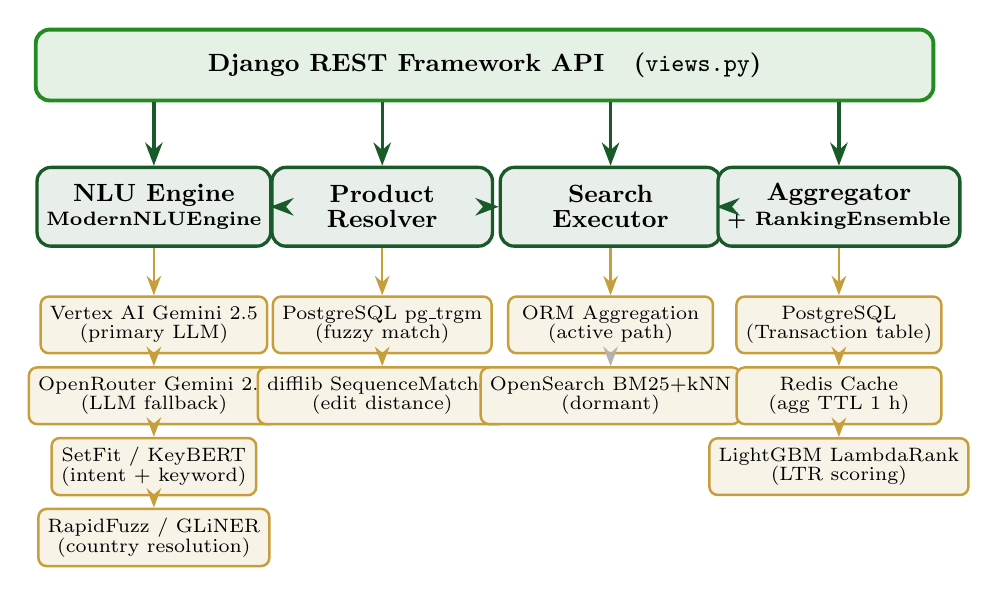
\begin{tikzpicture}[
  stage/.style={rectangle, rounded corners=5pt, draw=sectioncolor, fill=sectioncolor!10,
                minimum width=2.8cm, minimum height=1.0cm, align=center,
                font=\small\bfseries, line width=1.2pt},
  dep/.style={rectangle, rounded corners=3pt, draw=zaraigold!80, fill=zaraigold!10,
              minimum width=2.6cm, minimum height=0.72cm, align=center,
              font=\scriptsize, line width=0.9pt},
  api/.style={rectangle, rounded corners=5pt, draw=zaraigreen, fill=zaraigreen!12,
              minimum width=11.4cm, minimum height=0.9cm, align=center,
              font=\small\bfseries, line width=1.4pt},
  harr/.style={-Stealth, line width=1.2pt, color=sectioncolor},
  varr/.style={-Stealth, line width=0.9pt, color=zaraigold!80},
  farr/.style={-Stealth, dashed, line width=0.9pt, color=gray!60}
]

% ── Row 0: API Gateway (wide box across all 4 stages) ─────────────────────
\node[api] (apigw) at (4.2, 6.2)
      {Django REST Framework API\quad(\texttt{views.py})};

% ── Row 1: four pipeline stages ──────────────────────────────────────────
\node[stage] (nlu)  at (0,   4.4) {NLU Engine\\[-2pt]\scriptsize ModernNLUEngine};
\node[stage] (res)  at (2.9, 4.4) {Product\\[-2pt]Resolver};
\node[stage] (exec) at (5.8, 4.4) {Search\\[-2pt]Executor};
\node[stage] (agg)  at (8.7, 4.4) {Aggregator\\[-2pt]\scriptsize + RankingEnsemble};

% ── Arrows: API → stages ─────────────────────────────────────────────────
\draw[harr] (apigw.south -| nlu.north)  -- (nlu.north);
\draw[harr] (apigw.south -| res.north)  -- (res.north);
\draw[harr] (apigw.south -| exec.north) -- (exec.north);
\draw[harr] (apigw.south -| agg.north)  -- (agg.north);

% ── Arrows: stage → stage ────────────────────────────────────────────────
\draw[harr] (nlu.east)  -- (res.west);
\draw[harr] (res.east)  -- (exec.west);
\draw[harr] (exec.east) -- (agg.west);

% ── Row 2: dependencies (directly below each stage) ──────────────────────

%  NLU deps
\node[dep] (v1) at (0, 2.9)  {Vertex AI Gemini 2.5\\[-1pt]\scriptsize(primary LLM)};
\node[dep] (v2) at (0, 2.0)  {OpenRouter Gemini 2.0\\[-1pt]\scriptsize(LLM fallback)};
\node[dep] (v3) at (0, 1.1)  {SetFit / KeyBERT\\[-1pt]\scriptsize(intent + keyword)};
\node[dep] (v4) at (0, 0.2)  {RapidFuzz / GLiNER\\[-1pt]\scriptsize(country resolution)};

%  Resolver deps
\node[dep] (r1) at (2.9, 2.9) {PostgreSQL pg\_trgm\\[-1pt]\scriptsize(fuzzy match)};
\node[dep] (r2) at (2.9, 2.0) {difflib SequenceMatcher\\[-1pt]\scriptsize(edit distance)};

%  Executor deps
\node[dep] (e1) at (5.8, 2.9) {ORM Aggregation\\[-1pt]\scriptsize(active path)};
\node[dep] (e2) at (5.8, 2.0) {OpenSearch BM25+kNN\\[-1pt]\scriptsize(dormant)};

%  Aggregator deps
\node[dep] (a1) at (8.7, 2.9) {PostgreSQL\\[-1pt]\scriptsize(Transaction table)};
\node[dep] (a2) at (8.7, 2.0) {Redis Cache\\[-1pt]\scriptsize(agg TTL 1 h)};
\node[dep] (a3) at (8.7, 1.1) {LightGBM LambdaRank\\[-1pt]\scriptsize(LTR scoring)};

% ── Arrows: stages → their deps ──────────────────────────────────────────
\draw[varr] (nlu.south)  -- (v1.north);
\draw[varr] (v1.south)   -- (v2.north);
\draw[varr] (v2.south)   -- (v3.north);
\draw[varr] (v3.south)   -- (v4.north);

\draw[varr] (res.south)  -- (r1.north);
\draw[varr] (r1.south)   -- (r2.north);

\draw[varr] (exec.south) -- (e1.north);
\draw[farr] (e1.south)   -- (e2.north);   % dashed = dormant

\draw[varr] (agg.south)  -- (a1.north);
\draw[varr] (a1.south)   -- (a2.north);
\draw[varr] (a2.south)   -- (a3.north);

\end{tikzpicture}
\caption{ZaraiLink search engine component map. Solid gold arrows show active
dependencies; dashed arrow indicates a dormant path.}
\end{figure}

\subsection{Technology Stack}

\begin{table}[H]
\centering
\renewcommand{\arraystretch}{1.3}
\begin{tabularx}{\textwidth}{lXl}
\toprule
\rowcolor{tableheader!20}
\textbf{Layer} & \textbf{Technology} & \textbf{Role} \\
\midrule
Web framework      & Django 4.2 + Django REST Framework   & API endpoints, ORM \\
Database           & PostgreSQL (pg\_trgm extension)       & Primary data store \\
Cache              & Redis 7 / LocMemCache (fallback)      & NLU \& aggregation cache \\
LLM primary        & Vertex AI Gemini 2.5 Flash Lite       & Unified entity extraction \\
LLM fallback       & OpenRouter Gemini 2.0 Flash Lite      & LLM resilience \\
Intent classifier  & SetFit (HuggingFace)                  & Buy/Sell classification \\
Keyword extractor  & KeyBERT (paraphrase-MiniLM-L6-v2)    & Product keyword fallback \\
NER model          & GLiNER (urchade/gliner\_base)         & Zero-shot NER (optional) \\
Fuzzy matching     & RapidFuzz                             & Country name resolution \\
Ranker             & LightGBM LambdaRank                   & LTR scoring \\
Semantic search    & all-MiniLM-L6-v2 (FAISS HNSW)        & OpenSearch kNN (dormant) \\
\bottomrule
\end{tabularx}
\caption{Technology stack by layer}
\end{table}

\newpage
% ─────────────────────────────────────────────────────────────────────────────
\section{Stage 1: Natural Language Understanding Engine}
\label{sec:nlu}

\subsection{Overview}

The \texttt{ModernNLUEngine} class (file: \texttt{backend/search/services/nlu\_engine.py},
1,516 lines) converts a raw free-text query into a machine-readable intent structure.
It uses a \emph{hybrid} extraction strategy: cheap deterministic rules run first, an LLM
is consulted for the hard cases, and every component has a keyword-based or heuristic
fallback so parsing \emph{never blocks}.

\subsection{Fast Path: HS Code Detection}

Before any ML inference, the engine checks whether the query is a raw HS (Harmonised
System) tariff code.  Supported formats include dot-notation (\texttt{1702.3090}),
spaced (\texttt{1702 3090}) and hyphen-separated (\texttt{17-02-30-90}).  On a match the
query is normalised to canonical dot form and the full NLU pipeline is bypassed.

\subsection{Intent Detection Pipeline}

Intent classification determines whether a user is looking to \textbf{buy} (find suppliers)
or \textbf{sell} (find buyers).  The pipeline runs three sub-steps in priority order:

\begin{enumerate}
  \item \textbf{Semantic reversal rules} --- 182 longest-match phrase patterns that
        handle constructs such as
        \emph{``looking for sellers of X''} $\Rightarrow$ \texttt{BUY}, or
        \emph{``we export X''} $\Rightarrow$ \texttt{SELL}.
  \item \textbf{SetFit classifier} --- A SetFit model fine-tuned on 30 trade-domain
        labelled examples (\texttt{backend/search/models/intent\_model/}).  SetFit
        requires very few labelled examples due to contrastive sentence-pair pre-training.
  \item \textbf{Keyword regex fallback} --- Matches explicit cue words
        (\emph{buy, purchase, import, supplier, source} $\Rightarrow$ \texttt{BUY};
         \emph{sell, export, buyer, customer} $\Rightarrow$ \texttt{SELL}).
        If no cue is found the engine defaults to \texttt{BUY}, the more common query
        type for Pakistani importers.
\end{enumerate}

\subsection{LLM Unified Extraction}

A single LLM call (max 256 tokens) extracts the following entities simultaneously:

\begin{itemize}
  \item \textbf{Products} --- up to two product keywords as an array
  \item \textbf{Country} --- origin or destination country
  \item \textbf{Price signal} --- operator (\texttt{lte}/\texttt{gte}), numeric value,
        currency, and a ranking hint (\texttt{price\_asc} / \texttt{price\_desc})
  \item \textbf{Quantity} --- volume in metric tonnes if mentioned
\end{itemize}

\textbf{Primary LLM}: Vertex AI \texttt{gemini-2.5-flash-lite} (0.29\,s time-to-first-token).

\textbf{Fallback LLM}: OpenRouter \texttt{google/gemini-2.0-flash-lite} --- activated
automatically on Vertex API error, quota exhaustion or timeout.

\subsection{Product Keyword Resolution}

After the LLM call the extracted product string is further resolved via a four-step
cascade:

\begin{enumerate}
  \item \textbf{LLM output} --- used directly if a valid non-empty string.
  \item \textbf{KeyBERT} --- extracts the highest-scoring n-gram from the query using
        the sentence-transformer \texttt{paraphrase-MiniLM-L6-v2} with a 240-word stop
        list tuned for agricultural trade jargon.
  \item \textbf{Trigram similarity} --- if neither of the above yields a result,
        the query is matched directly against PostgreSQL's \texttt{pg\_trgm} index on
        \texttt{ProductSubCategory.name} (threshold 0.3).
  \item \textbf{Stop-word strip} --- strip all known stop phrases and take the
        longest remaining token.
\end{enumerate}

\subsection{Country Identification}

Country resolution uses three layers:

\begin{enumerate}
  \item \textbf{Dictionary lookup} --- 80+ countries in a hand-curated mapping keyed on
        common variants, abbreviations and Urdu-romanised names.
  \item \textbf{LLM cross-validation} --- the country returned by the LLM is
        reconciled with the dictionary to handle aliases.
  \item \textbf{RapidFuzz WRatio} --- fuzzy matching against the dictionary keys with
        an 80\% confidence threshold to handle OCR errors and non-standard spellings.
  \item \textbf{GLiNER NER} (optional, disabled by default) --- zero-shot span
        extraction using \texttt{urchade/gliner\_base} can be enabled with the
        \texttt{\_GLINER\_ENABLED} flag.
\end{enumerate}

\subsection{Scope Inference}

The \emph{scope} signals whether the user wants Pakistani trading partners only or
worldwide results:

\begin{table}[H]
\centering
\renewcommand{\arraystretch}{1.3}
\begin{tabular}{p{6cm}l}
\toprule
\rowcolor{tableheader!20}
\textbf{Signal} & \textbf{Inferred Scope} \\
\midrule
A non-Pakistani foreign country resolved & \texttt{worldwide} \\
Local city / Pakistani domain keyword    & \texttt{pakistan} \\
No geographic signal                     & Inherit from UI context \\
\bottomrule
\end{tabular}
\caption{Scope inference rules}
\end{table}

\subsection{NLU Output Schema}

The NLU engine returns a Python dict with the following guaranteed keys:

\begin{lstlisting}[caption={NLU output schema (Python)}]
{
    "intent":           "BUY" | "SELL",
    "product":          str,          # primary resolved keyword
    "product_keyword":  str,          # alias (same value)
    "product_keyword2": str,          # secondary product if two mentioned
    "country":          str | None,
    "quantity":         str | None,   # e.g. "1000 MT"
    "price_filter": {
        "range": {"usd_per_mt": {"lte"|"gte": float}},
        "ranking_hint": "price_asc" | "price_desc" | None
    },
    "os_filter":     {...},           # OpenSearch bool filter clauses
    "entities":      [...],           # GLiNER span extractions
    "ui_context":    "worldwide" | "pakistan",
    "is_hs_query":   bool
}
\end{lstlisting}

\subsection{NLU Caching}

\begin{itemize}
  \item \textbf{Cache key}: \texttt{"nlu\_" + MD5(query.lower() + ":" + scope.lower())}
  \item \textbf{TTL}: 24 hours
  \item \textbf{Backend}: Redis if reachable; LocMemCache otherwise.
\end{itemize}

\newpage
% ─────────────────────────────────────────────────────────────────────────────
\section{Stage 2: Product Resolution}
\label{sec:resolution}

\subsection{Overview}

Product resolution maps the NLU-extracted product keyword to a list of
\texttt{ProductSubCategory} primary keys, which are the anchors for all downstream
database queries.  The resolver also handles HS-code queries and multi-variant products.

\subsection{Five-Pass Matching Cascade}

\begin{table}[H]
\centering
\renewcommand{\arraystretch}{1.4}
\begin{tabularx}{\textwidth}{clXl}
\toprule
\rowcolor{tableheader!20}
\textbf{Pass} & \textbf{Method} & \textbf{Logic} & \textbf{Threshold} \\
\midrule
1 & Prefix (SubCategory)  & \texttt{ProductSubCategory.name \_\_istartswith} & exact \\
2 & Prefix (Item)         & \texttt{ProductItem.name \_\_istartswith} & exact \\
3 & Substring             & \texttt{icontains} on both tables & exact \\
4 & Trigram fuzzy         & PostgreSQL \texttt{TrigramSimilarity} & $> 0.30$ \\
5 & Edit distance         & Python \texttt{difflib.SequenceMatcher} & $\geq 0.75$ \\
6 & Needle-in-haystack    & Word-by-word token search for garbled queries & any token \\
\bottomrule
\end{tabularx}
\caption{Product resolution pass cascade}
\end{table}

\subsection{HS Code Resolution}

When the query is flagged as an HS-code query the resolver performs a cascade lookup
against \texttt{ProductSubCategory.hs\_code}:

\begin{enumerate}
  \item Exact match on normalised code (e.g.\ \texttt{1702.3090})
  \item Prefix match (\texttt{startswith}) to capture six-, four- and two-digit chapter
        codes
  \item Progressively shorter prefix to handle partial codes
\end{enumerate}

If more than \textbf{20} subcategory variants match the same chapter code, the engine
sets \texttt{needs\_disambiguation = True} and returns a variant picker payload to the
frontend rather than a result list.

\subsection{Scope-Aware Trade Type Mapping}

To prevent zero-result pages the resolver maps \emph{(intent, scope)} to a
\texttt{trade\_type} filter, since Pakistani customs data records each transaction from
the Pakistani importer's perspective:

\begin{table}[H]
\centering
\renewcommand{\arraystretch}{1.3}
\begin{tabular}{llll}
\toprule
\rowcolor{tableheader!20}
\textbf{Intent} & \textbf{Scope} & \textbf{Trade Type} & \textbf{Rationale} \\
\midrule
BUY  & pakistan  & EXPORT & Pakistani sellers exporting \\
SELL & pakistan  & IMPORT & Pakistani buyers importing \\
BUY  & worldwide & IMPORT & Foreign suppliers delivering to Pak \\
SELL & worldwide & EXPORT & Foreign buyers receiving from Pak \\
\bottomrule
\end{tabular}
\caption{Intent $\times$ scope $\rightarrow$ trade type mapping}
\end{table}

\subsection{Availability Check Cache}

Before executing the full aggregation query, a lightweight availability check is run to
confirm that at least one transaction exists for the resolved subcategories under the
selected trade type.

\begin{itemize}
  \item \textbf{Cache key}: \texttt{"avail\_" + MD5(subcat\_ids:trade\_type:country)}
  \item \textbf{TTL}: 1 hour
\end{itemize}

\newpage
% ─────────────────────────────────────────────────────────────────────────────
\section{Stage 3: Search Execution}
\label{sec:execution}

\subsection{Three-Path Execution Strategy}

The search executor chooses one of three query paths based on service availability:

\begin{figure}[H]
\centering
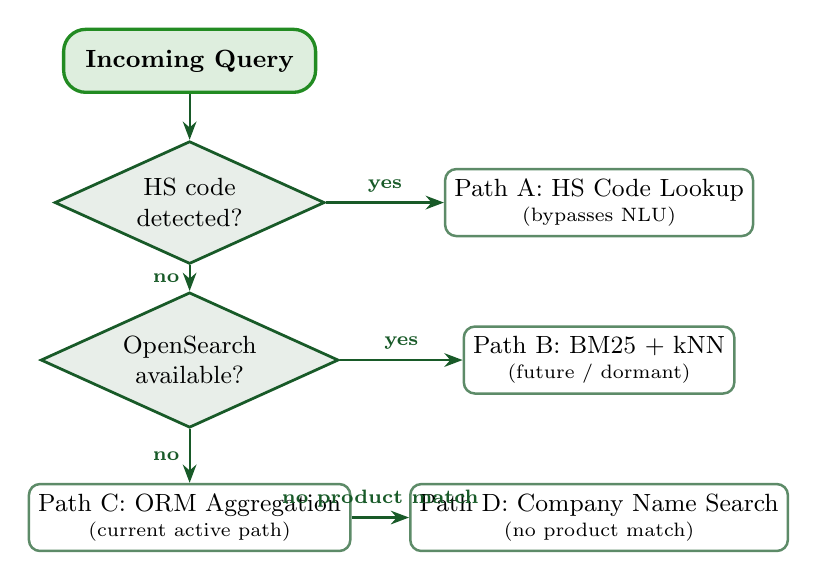
\begin{tikzpicture}[
  startstop/.style={rectangle, rounded corners=8pt, draw=zaraigreen, fill=zaraigreen!15,
                    minimum width=3.2cm, minimum height=0.8cm, align=center,
                    font=\small\bfseries, line width=1.2pt},
  decision/.style={diamond, draw=sectioncolor, fill=sectioncolor!10,
                   aspect=2.2, align=center, font=\small,
                   minimum width=2.6cm, minimum height=1.0cm, line width=1pt},
  process/.style={rectangle, rounded corners=4pt, draw=sectioncolor!70, fill=white,
                  minimum width=3.4cm, minimum height=0.85cm, align=center,
                  font=\small, line width=0.9pt},
  arr/.style={-Stealth, thick, color=sectioncolor}
]

  % Start
  \node[startstop] (start) at (0, 0)    {Incoming Query};

  % Decision 1
  \node[decision]  (d1)    at (0, -1.8) {HS code\\detected?};

  % Yes branch (right)
  \node[process]   (hs)    at (5.2, -1.8)
        {Path A: HS Code Lookup\\[-2pt]\scriptsize(bypasses NLU)};

  % Decision 2
  \node[decision]  (d2)    at (0, -3.8) {OpenSearch\\available?};

  % Yes branch (right)
  \node[process]   (osp)   at (5.2, -3.8)
        {Path B: BM25 + kNN\\[-2pt]\scriptsize(future / dormant)};

  % No → ORM
  \node[process]   (orm)   at (0, -5.8)
        {Path C: ORM Aggregation\\[-2pt]\scriptsize(current active path)};

  % Fallback (right of ORM)
  \node[process]   (cn)    at (5.2, -5.8)
        {Path D: Company Name Search\\[-2pt]\scriptsize(no product match)};

  % ── Arrows ────────────────────────────────────────────────────────────
  \draw[arr] (start) -- (d1);

  % d1 → right (yes)
  \draw[arr] (d1.east) -- node[above, font=\scriptsize\bfseries]{yes} (hs.west);

  % d1 → down (no)
  \draw[arr] (d1.south) -- node[left, font=\scriptsize\bfseries]{no} (d2.north);

  % d2 → right (yes)
  \draw[arr] (d2.east) -- node[above, font=\scriptsize\bfseries]{yes} (osp.west);

  % d2 → down (no / current)
  \draw[arr] (d2.south) -- node[left, font=\scriptsize\bfseries]{no} (orm.north);

  % orm → right (no product match)
  \draw[arr] (orm.east) -- node[above, font=\scriptsize\bfseries]{no product match} (cn.west);

\end{tikzpicture}
\caption{Search execution path selection. The current active path is Path~C (ORM
aggregation). Path~B (OpenSearch) is fully implemented but dormant pending cluster setup.}
\end{figure}

\subsection{Path A: ORM Aggregation (Active)}

The currently active path aggregates the \texttt{Transaction} table using Django ORM
with the following pipeline:

\begin{lstlisting}[caption={Core ORM aggregation query structure (simplified)}]
Transaction.objects
  .filter(
      sub_category_id__in=subcat_ids,
      trade_type=trade_type,
      **({"origin_country__icontains": country} if country else {}),
  )
  .values("seller" if intent=="BUY" else "buyer")
  .annotate(
      total_volume=Sum("qty_mt"),
      avg_price=Avg("usd_per_mt"),
      shipment_count=Count("id"),
      last_shipment_date=Max("reporting_date"),
  )
  .order_by("-total_volume")
\end{lstlisting}

Key design decisions:

\begin{itemize}
  \item Grouping is by \textbf{company name} rather than a surrogate key because the
        same physical company may appear under slightly varying spellings across
        transaction records.
  \item A \textbf{post-aggregation price filter} (equivalent to an SQL \texttt{HAVING}
        clause) applies the NLU price constraint after the \texttt{avg\_price} annotation
        has been computed.
\end{itemize}

\subsection{Path B: OpenSearch Hybrid (Dormant)}

The OpenSearch path is fully implemented but currently disabled via a compile-time flag
in \texttt{search\_service.py} (line~232).  When enabled it issues a hybrid query:

\begin{itemize}
  \item \textbf{BM25 text search} with per-field boosts:
        \texttt{clean\_product\_name}$\times 9$,
        \texttt{sub\_category\_name}$\times 7$,
        \texttt{product\_item\_name}$\times 5$,
        \texttt{buyer}/\texttt{seller}$\times 1$.
  \item \textbf{kNN dense retrieval} using 384-dimensional sentence embeddings
        (\texttt{all-MiniLM-L6-v2}), indexed as FAISS HNSW in the
        \texttt{trade\_index} index.
  \item Scores are fused via OpenSearch's native \texttt{bool.should} with
        tunable weights.
\end{itemize}

The index is populated by the management command
\texttt{python manage.py sync\_search} (344 lines, \texttt{sync\_search.py}).

\subsection{Path C: Company-Name Fallback}

When the five-pass product resolver returns no subcategory matches \emph{and} the
stripped query token is at least three characters long, the executor performs a direct
\texttt{icontains} search against \texttt{Transaction.seller} and
\texttt{Transaction.buyer}.  Duplicate company names are deduplicated and returned as
lightweight company profiles.

\subsection{Search Request Parameters}

\begin{table}[H]
\centering
\renewcommand{\arraystretch}{1.3}
\begin{tabularx}{\textwidth}{llX}
\toprule
\rowcolor{tableheader!20}
\textbf{Parameter} & \textbf{Type} & \textbf{Description} \\
\midrule
\texttt{q}            & string   & Raw natural-language query \\
\texttt{scope}        & enum     & \texttt{worldwide} or \texttt{pakistan}; UI context \\
\texttt{hs\_code}     & string   & Optional direct HS code lookup, bypasses NLU \\
\texttt{subcat\_id}   & integer  & Optional resolved subcategory ID, bypasses resolution \\
\texttt{variant\_name}& string   & Optional exact product variant name filter \\
\bottomrule
\end{tabularx}
\caption{GET /api/search/ request parameters}
\end{table}

\newpage
% ─────────────────────────────────────────────────────────────────────────────
\section{Stage 4: Aggregation, Intelligence \& Ranking}
\label{sec:ranking}

\subsection{SupplierAggregator}

The \texttt{SupplierAggregator} class (\texttt{backend/search/services/aggregation.py},
654 lines) provides three public methods:

\begin{description}[leftmargin=2.5cm]
  \item[\texttt{get\_suppliers\_for\_subcategories()}] Main search result aggregation.
        Groups transactions by company, computes volume/price/recency, applies
        volume-fit scoring if a quantity signal is present.

  \item[\texttt{get\_supplier\_details()}] Deep-dive for a single seller.
        Returns monthly sparklines, shipment-size distribution, buyer insights and a
        full transaction history (top 50 records).

  \item[\texttt{get\_buyer\_details()}] Symmetrical to supplier details for the
        \texttt{SELL} intent flow.  Shows purchase patterns, supplier relationships and
        order-size distribution.
\end{description}

\subsection{Intelligence Metrics}

The \texttt{\_calculate\_intelligence()} method computes four dynamic signals from
the raw transaction data:

\begin{table}[H]
\centering
\renewcommand{\arraystretch}{1.4}
\begin{tabularx}{\textwidth}{lX}
\toprule
\rowcolor{tableheader!20}
\textbf{Signal} & \textbf{Definition} \\
\midrule
\textbf{Repeat Ratio} &
  Fraction of transactions involving counterparties that appear more than once.
  Indicates relationship stability. \\
\textbf{Concentration Ratio} &
  Percentage of total volume accounted for by the top-3 counterparties.
  High concentration = single-customer risk. \\
\textbf{Pricing Label} &
  Categorical label derived from average unit price vs.\ market median.
  Labels: \emph{Premium / Competitive / Stable} (seller); \\
  & \emph{Opportunistic / Sensitive / Stable} (buyer). \\
\textbf{Momentum Label} &
  Volume trend direction vs.\ dataset maximum date.
  Labels: \emph{Growing / Stable / Declining}. \\
\textbf{Generated Summary} &
  Human-readable one-sentence insight synthesising the above signals. \\
\bottomrule
\end{tabularx}
\caption{Per-company intelligence signals}
\end{table}

\subsection{Volume-Fit Scoring}

When the query contains a quantity signal (e.g.\ \emph{``1000 MT of sugar''}), each
company is scored on its ability to fulfil that order:

\begin{equation}
  s_{\text{vol}} = 0.5 \cdot \min\!\left(\frac{V_{\max}}{Q},\,1\right)
                 + 0.3 \cdot \min\!\left(\frac{V_{\text{total}}}{Q},\,1\right)
                 + 0.2 \cdot \min\!\left(\frac{\bar{V}}{Q},\,1\right)
  \label{eq:volfit}
\end{equation}

where $V_{\max}$ is the largest single shipment, $V_{\text{total}}$ the company's
cumulative volume, $\bar{V}$ the average shipment size, and $Q$ the requested quantity.
The score is binned into four labels:

\begin{center}
\begin{tabular}{cc}
\toprule
\rowcolor{tableheader!20}
$s_{\text{vol}}$ range & Label \\
\midrule
$\geq 0.80$ & \emph{Strong} \\
$\geq 0.50$ & \emph{Good} \\
$\geq 0.30$ & \emph{Partial} \\
$< 0.30$    & \emph{Low} \\
\bottomrule
\end{tabular}
\end{center}

\subsection{Intent-Aware Composite Ranking}

Each company receives a composite relevance score computed from four normalised signals:

\begin{equation}
  \text{score} = w_1 \hat{V} + w_2 \hat{C} + w_3 \hat{P} + w_4 \hat{R}
  \label{eq:score}
\end{equation}

where $\hat{V}$, $\hat{C}$, $\hat{P}$, $\hat{R}$ are min-max normalised values of
\emph{total volume}, \emph{shipment count}, \emph{inverse unit price} (lower price
scores higher) and \emph{recency date} respectively.

The weight vector is selected by the NLU \texttt{ranking\_hint}:

\begin{table}[H]
\centering
\renewcommand{\arraystretch}{1.3}
\begin{tabular}{lccccl}
\toprule
\rowcolor{tableheader!20}
\textbf{Hint} & $w_1$ (vol) & $w_2$ (count) & $w_3$ (price) & $w_4$ (recency) & \textbf{Trigger} \\
\midrule
\texttt{price\_asc}  & 0.15 & 0.15 & 0.50 & 0.20 & cheap, affordable, budget \\
\texttt{price\_desc} & 0.45 & 0.25 & 0.05 & 0.25 & bulk, premium, large order \\
\emph{default}       & 0.35 & 0.25 & 0.15 & 0.25 & no price signal \\
\bottomrule
\end{tabular}
\caption{Composite ranking weight presets}
\end{table}

\textbf{Price handling edge case}: when \texttt{avg\_price} is zero (unknown) and the
hint is \emph{not} \texttt{price\_asc}, the price term contributes a neutral
$w_3 \times 0.5$ rather than zero to avoid penalising companies with missing price data.

\subsection{Aggregation Cache}

\begin{itemize}
  \item \textbf{Cache key}: \texttt{"agg\_" + MD5(subcat\_ids:intent:scope:country:price:product\_items)}
  \item \textbf{TTL}: 1 hour
  \item \textbf{Backend}: Redis / LocMemCache fallback
\end{itemize}

\newpage
% ─────────────────────────────────────────────────────────────────────────────
\section{API Endpoints}
\label{sec:api}

All endpoints are served under the \texttt{/api/search/} prefix and use Django REST
Framework's JSON renderer.  Authentication is session-based.

\subsection{Main Search --- \texttt{GET /api/search/}}

\begin{infobox}
\textbf{URL}: \texttt{GET /api/search/?q=\{query\}\&scope=\{scope\}}
\end{infobox}

\textbf{Response schema}:

\begin{lstlisting}[caption={Search response schema}]
{
    "query":               "<original user input>",
    "parsed_query":        { /* full NLU result */ },
    "needs_disambiguation": false,
    "is_broad_search":     false,
    "variants":            [],
    "results": [
        {
            "name":              "Ningbo Trading Co.",
            "country":           "China",
            "total_volume":      12500.5,      // metric tonnes
            "avg_price":         650.25,       // USD per MT
            "shipment_count":    45,
            "last_shipment_date":"2023-12-15",
            "avg_shipment_vol":  277.8,        // MT per shipment
            "type":              "Supplier",   // or "Buyer"
            "relevance_score":   0.8742,
            "volume_fit":        "Strong"      // or N/A
        }
    ],
    "market_snapshot": {
        "total_count":      12,
        "avg_price_global": 645.33,  // volume-weighted market average
        "top_country":      "China"
    },
    "count":         12,
    "search_engine": "orm"   // or "opensearch"
}
\end{lstlisting}

\subsection{Autocomplete --- \texttt{GET /api/search/autocomplete/}}

\begin{infobox}
\textbf{URL}: \texttt{GET /api/search/autocomplete/?q=\{prefix\}}\\
Returns up to 8 \texttt{ProductSubCategory} suggestions ranked by total trade volume,
with labels displaying volume in metric tonnes.
\end{infobox}

\subsection{Supplier Detail --- \texttt{GET /api/search/supplier-detail/}}

\begin{infobox}
\textbf{URL}: \texttt{GET /api/search/supplier-detail/?name=\{company\}\&query=\{q\}\&scope=\{scope\}}\\
Returns full deep-dive including monthly volume/price sparklines, shipment-size
bucket chart, unique buyer count, top transactions (up to 50) and intelligence signals.
\end{infobox}

\subsection{Supplier Compare --- \texttt{GET /api/search/compare/}}

\begin{infobox}
\textbf{URL}: \texttt{GET /api/search/compare/?suppliers=A,B,C\&query=\{q\}}\\
Returns a side-by-side comparison object for up to three companies, including price
ranges, volume sparklines, shipment date ranges and destination country breakdowns.
\end{infobox}

\newpage
% ─────────────────────────────────────────────────────────────────────────────
\section{Caching Architecture}
\label{sec:caching}

\subsection{Cache Backend Selection}

The platform uses a two-tier fallback strategy for its cache backend:

\begin{enumerate}
  \item \textbf{Redis} --- preferred backend, auto-detected on
        \texttt{127.0.0.1:6379}.  If a connection can be established at startup,
        the Django cache backend is set to \texttt{django-redis}.
  \item \textbf{LocMemCache} --- in-process Python dict used when Redis is
        unavailable.  Not shared between processes and not persistent across restarts,
        but guarantees that caching \emph{never fails}.
\end{enumerate}

\subsection{Cache Hierarchy}

\begin{table}[H]
\centering
\renewcommand{\arraystretch}{1.3}
\begin{tabularx}{\textwidth}{llXl}
\toprule
\rowcolor{tableheader!20}
\textbf{Cache Name} & \textbf{Key Prefix} & \textbf{Covers} & \textbf{TTL} \\
\midrule
NLU cache           & \texttt{nlu\_}  &
  Parsed intent struct for a given (query, scope) pair & 24 h \\
Availability check  & \texttt{avail\_} &
  Whether any transactions exist for (subcat\_ids, trade\_type, country) & 1 h \\
Aggregation cache   & \texttt{agg\_} &
  Full ranked supplier/buyer list for a given parameter set & 1 h \\
\bottomrule
\end{tabularx}
\caption{Cache tiers and TTLs}
\end{table}

\subsection{Cache Key Construction}

All cache keys are deterministic MD5 hashes of the relevant parameter tuple, making
them collision-resistant and length-bounded:

\begin{lstlisting}[caption={Cache key construction pattern}]
import hashlib

def _make_key(prefix: str, *parts) -> str:
    raw = ":".join(str(p) for p in parts)
    return prefix + hashlib.md5(raw.encode()).hexdigest()

# Examples
nlu_key  = _make_key("nlu_",  query.lower(), scope.lower())
agg_key  = _make_key("agg_",  subcat_ids, intent, scope, country,
                               price, product_items)
avail_key = _make_key("avail_", subcat_ids, trade_type, country)
\end{lstlisting}

\newpage
% ─────────────────────────────────────────────────────────────────────────────
\section{Machine Learning Models}
\label{sec:ml}

\subsection{Model Inventory}

\begin{table}[H]
\centering
\renewcommand{\arraystretch}{1.4}
\begin{tabularx}{\textwidth}{>{\raggedright}p{3.8cm}>{\raggedright}p{3.2cm}X>{\raggedright\arraybackslash}p{2.0cm}}
\toprule
\rowcolor{tableheader!20}
\textbf{Model} & \textbf{Type} & \textbf{Role} & \textbf{Status} \\
\midrule
SetFit intent classifier &
  Few-shot contrastive fine-tune &
  Buy/Sell intent classification (30 examples) &
  Active \\
KeyBERT (paraphrase-MiniLM-L6-v2) &
  Sentence-transformer + BERT &
  Product keyword extraction fallback &
  Active \\
GLiNER (urchade/gliner\_base) &
  Zero-shot NER &
  Country/entity span extraction &
  Disabled \\
LightGBM LambdaRank &
  Gradient-boosted trees &
  LTR re-ranking of aggregated results &
  Active \\
all-MiniLM-L6-v2 (FAISS HNSW) &
  Sentence-transformer &
  384-dim dense retrieval index &
  Dormant \\
Vertex AI Gemini 2.5 Flash Lite &
  LLM (API) &
  Unified entity extraction &
  Active \\
OpenRouter Gemini 2.0 Flash Lite &
  LLM (API) &
  LLM fallback &
  Active (fallback) \\
\bottomrule
\end{tabularx}
\caption{ML model inventory}
\end{table}

\subsection{SetFit Intent Classifier}

SetFit (\emph{Sentence Fine-Tuning}) is a parameter-efficient classification paradigm
that first fine-tunes a sentence-transformer via contrastive learning on a small set of
labelled pairs, then trains a lightweight head on the resulting embeddings.

\begin{itemize}
  \item \textbf{Training set}: 30 trade-domain sentences per class (BUY / SELL)
  \item \textbf{Model artefact}: \texttt{backend/search/models/intent\_model/}
  \item \textbf{Inference latency}: $<5$\,ms (CPU)
\end{itemize}

\subsection{LightGBM LambdaRank}

The LTR model (\texttt{backend/search/models/lgbm\_ltr.txt}) provides a learned
relevance signal used to supplement the heuristic composite score.

\begin{itemize}
  \item \textbf{Algorithm}: LambdaRank (listwise, NDCG-optimised)
  \item \textbf{Features}: normalised volume, shipment count, recency, price signal,
        country match, volume-fit score
  \item \textbf{Integration}: 30\% weight in the final ensemble
        (\texttt{0.7 $\times$ heuristic + 0.3 $\times$ LightGBM})
\end{itemize}

\subsection{KeyBERT Keyword Extraction}

KeyBERT uses the sentence-transformer \texttt{paraphrase-MiniLM-L6-v2} to score
candidate n-grams by cosine similarity to the full query embedding.  A 240-word stop
list filters out supply-chain meta-language (``importer'', ``looking for'', ``cheap'',
``kg'') so the model focuses on the product noun phrase.

\newpage
% ─────────────────────────────────────────────────────────────────────────────
\section{Resilience \& Fallback Design}
\label{sec:resilience}

A core design principle of the ZaraiLink search engine is that \textbf{no single
component failure should return an error to the user}.  Every external dependency has a
deterministic fallback:

\begin{table}[H]
\centering
\renewcommand{\arraystretch}{1.4}
\begin{tabularx}{\textwidth}{lXX}
\toprule
\rowcolor{tableheader!20}
\textbf{Component} & \textbf{Failure Mode} & \textbf{Fallback} \\
\midrule
Vertex AI (LLM primary) &
  API error, quota, timeout &
  OpenRouter LLM \\
OpenRouter (LLM fallback) &
  API error &
  KeyBERT + regex + dict \\
SetFit classifier &
  Model file missing &
  Keyword regex rules \\
KeyBERT &
  Model file missing &
  Stop-word strip heuristic \\
GLiNER NER &
  Disabled by default &
  Dict lookup + RapidFuzz \\
Redis cache &
  Connection refused &
  LocMemCache (in-process) \\
OpenSearch &
  Disabled / unreachable &
  ORM aggregation path \\
Product resolver (no match) &
  Zero subcategory matches &
  Company-name icontains search \\
\bottomrule
\end{tabularx}
\caption{Failure modes and fallbacks}
\end{table}

The OpenSearch client is configured with a \textbf{3-second timeout} to ensure fast
failure in case the cluster is temporarily unresponsive.  The ORM fallback is triggered
silently; the response includes a \texttt{"search\_engine": "orm"} field to assist
debugging.

\newpage
% ─────────────────────────────────────────────────────────────────────────────
\section{Logging \& Observability}
\label{sec:logging}

\subsection{Logger Configuration}

The \texttt{search} logger is configured at \texttt{INFO} level with a console
(stdout) handler.  No structured logging aggregator is connected in the current
deployment; logs are captured by the hosting platform's stdout stream.

\subsection{Log Namespaces}

\begin{table}[H]
\centering
\renewcommand{\arraystretch}{1.3}
\begin{tabularx}{\textwidth}{lX}
\toprule
\rowcolor{tableheader!20}
\textbf{Prefix} & \textbf{Events logged} \\
\midrule
\texttt{[NLU]}        & Intent, product keyword, country, price extracted per query \\
\texttt{[TIMING NLU]} & Per-subsystem latency (LLM call, KeyBERT, fuzzy matching) \\
\texttt{[CACHE]}      & Hit / miss notifications with key prefix \\
\texttt{[Ranking]}    & Weight preset selected (\texttt{price\_asc} / \texttt{price\_desc} / default) \\
\texttt{[Search]}     & Query dispatched, path selected (ORM / OpenSearch / company fallback) \\
\bottomrule
\end{tabularx}
\caption{Log namespace reference}
\end{table}

\newpage
% ─────────────────────────────────────────────────────────────────────────────
\section{Database Schema Interaction}
\label{sec:db}

\subsection{Core Tables Used}

\begin{table}[H]
\centering
\renewcommand{\arraystretch}{1.3}
\begin{tabularx}{\textwidth}{lXl}
\toprule
\rowcolor{tableheader!20}
\textbf{Table (Django model)} & \textbf{Key Columns} & \textbf{Used by} \\
\midrule
\texttt{Transaction} &
  \texttt{seller}, \texttt{buyer}, \texttt{qty\_mt}, \texttt{usd\_per\_mt},
  \texttt{trade\_type}, \texttt{reporting\_date}, \texttt{origin\_country},
  \texttt{destination\_country}, \texttt{hs\_code}, \texttt{tx\_reference} &
  Stages 3, 4 \\[4pt]
\texttt{ProductSubCategory} &
  \texttt{name}, \texttt{hs\_code}, \texttt{category\_id} &
  Stages 1, 2 \\[4pt]
\texttt{ProductItem} &
  \texttt{name}, \texttt{sub\_category\_id} &
  Stage 2 \\
\bottomrule
\end{tabularx}
\caption{Database tables accessed by the search engine}
\end{table}

\subsection{PostgreSQL Extensions Required}

The product resolver's trigram fuzzy matching requires the \texttt{pg\_trgm} extension:

\begin{lstlisting}[language=SQL, caption={pg\_trgm installation}]
-- Run once as superuser
CREATE EXTENSION IF NOT EXISTS pg_trgm;
\end{lstlisting}

The extension enables \texttt{TrigramSimilarity} and \texttt{GinIndex} on
\texttt{ProductSubCategory.name} and \texttt{ProductItem.name}, which are exploited
by Django's \texttt{TrigramSimilarity} database function in pass~4 of the resolver.

\newpage
% ─────────────────────────────────────────────────────────────────────────────
\section{End-to-End Query Walkthrough}
\label{sec:walkthrough}

This section traces a representative query through all four pipeline stages.

\begin{infobox}
\textbf{Example query}: \emph{``I want to buy cheap refined sugar under \$500 from Brazil''}\\
\textbf{UI context}: \texttt{worldwide}
\end{infobox}

\subsection{Stage 1: NLU}

\begin{enumerate}
  \item \textbf{HS fast path}: No HS code pattern found.
  \item \textbf{Semantic reversal}: ``I want to buy'' matches \texttt{BUY} pattern.
        SetFit confirms \texttt{BUY} with high confidence.
  \item \textbf{LLM unified extraction}:
        \texttt{products=["refined sugar"]},
        \texttt{country="Brazil"},
        \texttt{price=\{operator:"lte", value:500, currency:"USD", ranking\_hint:"price\_asc"\}}.
  \item \textbf{Scope inference}: \texttt{country="Brazil"} $\notin$ Pakistan set
        $\Rightarrow$ \texttt{scope="worldwide"}.
  \item \textbf{NLU output}:
        \texttt{intent=BUY, product="refined sugar", country="Brazil",}\\
        \texttt{price\_filter.range=\{usd\_per\_mt:\{lte:500\}\}, ranking\_hint="price\_asc"}.
\end{enumerate}

\subsection{Stage 2: Product Resolution}

\begin{enumerate}
  \item Pass 1 (prefix): ``refined sugar'' matches \texttt{ProductSubCategory} names
        starting with ``refined sugar'' $\Rightarrow$ IDs \{42, 44, 47\}.
  \item Trade type mapping: \texttt{BUY} $\times$ \texttt{worldwide}
        $\Rightarrow$ \texttt{trade\_type=IMPORT}.
  \item Availability check: cache miss; query confirms transactions exist.
\end{enumerate}

\subsection{Stage 3: Search Execution}

ORM path executes:

\begin{lstlisting}[caption={Effective SQL (paraphrased)}]
SELECT seller,
       SUM(qty_mt)         AS total_volume,
       AVG(usd_per_mt)     AS avg_price,
       COUNT(*)            AS shipment_count,
       MAX(reporting_date) AS last_shipment_date
FROM   trade_data_transaction
WHERE  sub_category_id IN (42, 44, 47)
  AND  trade_type = 'IMPORT'
  AND  origin_country ILIKE '%Brazil%'
GROUP BY seller
HAVING AVG(usd_per_mt) <= 500   -- post-aggregation price filter
ORDER BY total_volume DESC;
\end{lstlisting}

\subsection{Stage 4: Aggregation \& Ranking}

\begin{enumerate}
  \item \textbf{Weight preset}: \texttt{ranking\_hint="price\_asc"} selects
        $(w_1, w_2, w_3, w_4) = (0.15, 0.15, 0.50, 0.20)$.
  \item \textbf{Min-max normalisation}: applied per signal across all returned rows.
  \item \textbf{Score}: $\text{score} = 0.15\hat{V} + 0.15\hat{C} + 0.50\hat{P} + 0.20\hat{R}$
        where $\hat{P} = \widehat{1/\text{price}}$ (inverted so cheaper = higher score).
  \item \textbf{Output}: Ranked list of Brazilian refined-sugar exporters, sorted
        by composite score descending.  Top result will be the cheapest,
        most frequent, most recently active supplier.
\end{enumerate}

\subsection{Response}

\begin{lstlisting}[caption={Abbreviated API response}]
{
    "query": "I want to buy cheap refined sugar under $500 from Brazil",
    "parsed_query": {
        "intent": "BUY", "product": "refined sugar",
        "country": "Brazil", "ui_context": "worldwide",
        "price_filter": {"range": {"usd_per_mt": {"lte": 500}},
                         "ranking_hint": "price_asc"}
    },
    "results": [
        {"name": "Sao Paulo Acucar Ltda.", "country": "Brazil",
         "total_volume": 8400.0, "avg_price": 412.50,
         "shipment_count": 28, "relevance_score": 0.921}
    ],
    "market_snapshot": {"avg_price_global": 423.8, "top_country": "Brazil"},
    "count": 7, "search_engine": "orm"
}
\end{lstlisting}

\newpage
% ─────────────────────────────────────────────────────────────────────────────
\section{Source Code Structure}
\label{sec:code}

\begin{table}[H]
\centering
\renewcommand{\arraystretch}{1.3}
\begin{tabularx}{\textwidth}{lrX}
\toprule
\rowcolor{tableheader!20}
\textbf{File} & \textbf{Lines} & \textbf{Responsibility} \\
\midrule
\texttt{search/services/nlu\_engine.py}   & 1,516 &
  Full NLU with 5-stage extraction, LLM integration, caching \\
\texttt{search/services/search\_service.py} & 945 &
  Pipeline orchestration, product resolver, execution paths, ranking \\
\texttt{search/services/aggregation.py}   & 654 &
  ORM aggregation, intelligence scoring, volume-fit, sparklines \\
\texttt{search/views.py}                  & 271 &
  DRF API endpoints, request parsing, response serialisation \\
\texttt{search/management/commands/sync\_search.py} & 344 &
  OpenSearch index builder (management command) \\
\texttt{search/urls.py}                   & 29 &
  URL routing for all search endpoints \\
\bottomrule
\end{tabularx}
\caption{Search module source files}
\end{table}

\begin{table}[H]
\centering
\renewcommand{\arraystretch}{1.3}
\begin{tabularx}{\textwidth}{lX}
\toprule
\rowcolor{tableheader!20}
\textbf{Model Artefact} & \textbf{Description} \\
\midrule
\texttt{search/models/intent\_model/}  &
  SetFit fine-tuned checkpoint (HuggingFace format) \\
\texttt{search/models/lgbm\_ltr.txt}  &
  LightGBM LambdaRank trained model (text format) \\
\texttt{search\_index.pkl}            &
  Pickled in-memory search index (alternative to OpenSearch) \\
\bottomrule
\end{tabularx}
\caption{Model artefacts}
\end{table}

\newpage
% ─────────────────────────────────────────────────────────────────────────────
\section{Configuration \& Deployment Notes}
\label{sec:config}

\subsection{Environment Variables}

\begin{table}[H]
\centering
\renewcommand{\arraystretch}{1.3}
\begin{tabularx}{\textwidth}{lX}
\toprule
\rowcolor{tableheader!20}
\textbf{Variable} & \textbf{Purpose} \\
\midrule
\texttt{OPENAI\_API\_KEY}           & OpenAI API key (text-embedding-3-small, gpt-4o-mini) \\
\texttt{GOOGLE\_APPLICATION\_CREDENTIALS} &
  Path to service account JSON for Vertex AI Gemini \\
\texttt{OPENROUTER\_API\_KEY}       & OpenRouter API key (LLM fallback) \\
\texttt{REDIS\_URL}                 & Redis connection string; defaults to \texttt{redis://127.0.0.1:6379/1} \\
\texttt{OPENSEARCH\_HOST}           & OpenSearch cluster host (optional) \\
\texttt{DEBUG}                      & Django debug flag; hardcoded \texttt{True} in dev \\
\bottomrule
\end{tabularx}
\caption{Relevant environment variables}
\end{table}

\subsection{Development Setup}

\begin{itemize}
  \item Backend: \texttt{http://localhost:8000} (Django dev server)
  \item Frontend: \texttt{http://localhost:3000} (Create React App)
  \item Database: PostgreSQL local, \texttt{user=postgres}, \texttt{db=zarailink}
  \item Redis: optional, auto-detected on \texttt{127.0.0.1:6379}
\end{itemize}

\subsection{Required PostgreSQL Extension}

\begin{verbatim}
  psql -U postgres -d zarailink -c "CREATE EXTENSION IF NOT EXISTS pg_trgm;"
\end{verbatim}

\subsection{Enabling OpenSearch}

To activate the OpenSearch hybrid path:
\begin{enumerate}
  \item Deploy an OpenSearch cluster and set \texttt{OPENSEARCH\_HOST}.
  \item Run \texttt{python manage.py sync\_search} to build the \texttt{trade\_index}.
  \item Change the compile-time flag on line~232 of \texttt{search\_service.py}:
\end{enumerate}

\begin{lstlisting}[caption={Enabling OpenSearch path}]
# search_service.py, line 232
USE_OPENSEARCH = True   # was False
\end{lstlisting}

\newpage
% ─────────────────────────────────────────────────────────────────────────────
\section{Key Design Decisions}
\label{sec:decisions}

\begin{enumerate}
  \item \textbf{Single LLM call for all entities.}
        Rather than making separate API calls for product, country and price extraction,
        a single structured prompt extracts all three in one round trip (max 256 tokens).
        This keeps per-query LLM cost under \$0.0002 on Gemini 2.5 Flash Lite.

  \item \textbf{Group by company name, not ID.}
        Pakistani customs data does not have stable company identifiers across datasets;
        grouping by normalised company name avoids artificial fragmentation of the same
        trading entity.

  \item \textbf{Intent $\times$ scope $\rightarrow$ trade type mapping.}
        Explicitly mapping intent to the correct \texttt{trade\_type} filter is the
        single most important correctness decision: querying the wrong trade type
        silently returns zero results.

  \item \textbf{Post-aggregation price filter.}
        Applying the price constraint as a \texttt{HAVING}-equivalent after
        \texttt{AVG(usd\_per\_mt)} is computed means the filter operates on a
        representative average rather than on noisy individual transaction prices.

  \item \textbf{Asymmetric weight presets.}
        Giving price a 50\% weight for bargain queries and only 5\% for bulk/premium
        queries reflects real buyer behaviour: cost-sensitive importers care first about
        price; volume traders care first about proven capacity.

  \item \textbf{Graceful model degradation.}
        The SetFit, KeyBERT and GLiNER models are all loaded with try/except guards.
        If any model artefact is missing the system falls through to a faster, cheaper
        heuristic rather than raising an exception.
\end{enumerate}

% ─────────────────────────────────────────────────────────────────────────────
\section{Future Work}
\label{sec:future}

\begin{enumerate}
  \item \textbf{Activate OpenSearch hybrid path.}
        Enabling BM25+kNN retrieval would improve recall for long-tail agricultural
        product names that are not in the \texttt{ProductSubCategory} table.

  \item \textbf{Enable GLiNER NER.}
        Zero-shot span extraction would improve country resolution for uncommon country
        names and compound geography expressions (e.g.\ ``sub-Saharan Africa'').

  \item \textbf{Structured logging + metrics.}
        Integrating OpenTelemetry would expose per-stage latency histograms and
        cache-hit ratios as Prometheus metrics, enabling SLO-based alerting.

  \item \textbf{Continuous LTR retraining.}
        Collecting implicit feedback (click-through rate, contact-unlock events) and
        feeding it into periodic LightGBM retraining would improve ranking over time
        without manual labelling.

  \item \textbf{Multilingual query support.}
        Adding Urdu-script query normalisation (Nastaliq to Latin transliteration) would
        serve traders who type in their native script.
\end{enumerate}

% ─────────────────────────────────────────────────────────────────────────────
\section{Conclusion}

The ZaraiLink search engine is a purpose-built agricultural trade discovery system that
combines deterministic rule-based NLU, lightweight ML classifiers, LLM-powered entity
extraction and ORM-level database aggregation into a resilient, sub-second query
pipeline.

Its most important property is \emph{correctness under degradation}: the system makes
deliberate, conservative choices at every stage (defaulting to the BUY intent, applying
the correct trade-type filter, falling back to ORM when distributed search is
unavailable) to ensure that users always receive meaningful results even when individual
infrastructure components are offline.

With the OpenSearch hybrid path and continuous LTR retraining activated, the platform is
well-positioned to scale to larger product catalogues and higher query volumes while
maintaining the contextual accuracy that differentiates it from generic keyword search.

% ─────────────────────────────────────────────────────────────────────────────
\end{document}
